\section{Linux Network Stack}

\subsection{\shinfo}
The sk\_buff is a common data structure that is used in the Linux network stack to hold information for representing a packet and is used by many network card drivers. Basically, sk\_buff contains the packet’s metadata (e.g., its size and the protocol that uses this packet) and several pointers to different locations in the data itself, which is usually located in a different page (see Figure \ref{fig:sh_info}). The network stack supports packet cloning by copying sk buff metadata and letting the new one point to the same data as the old one. To support this data sharing, the skb shared info metadata structure is located in a row with the data. Just as in the previous attack, skb shared info is accidentally mapped for the device with the permissions of the packet (i.e., write for RX packets and read for TX packets). The main difference between this and the previous attack is that since the packet is either TX or RX, but never both, we cannot deduce the virtual address of the packet as we did in the previous case.

\begin{figure}
    \centering
    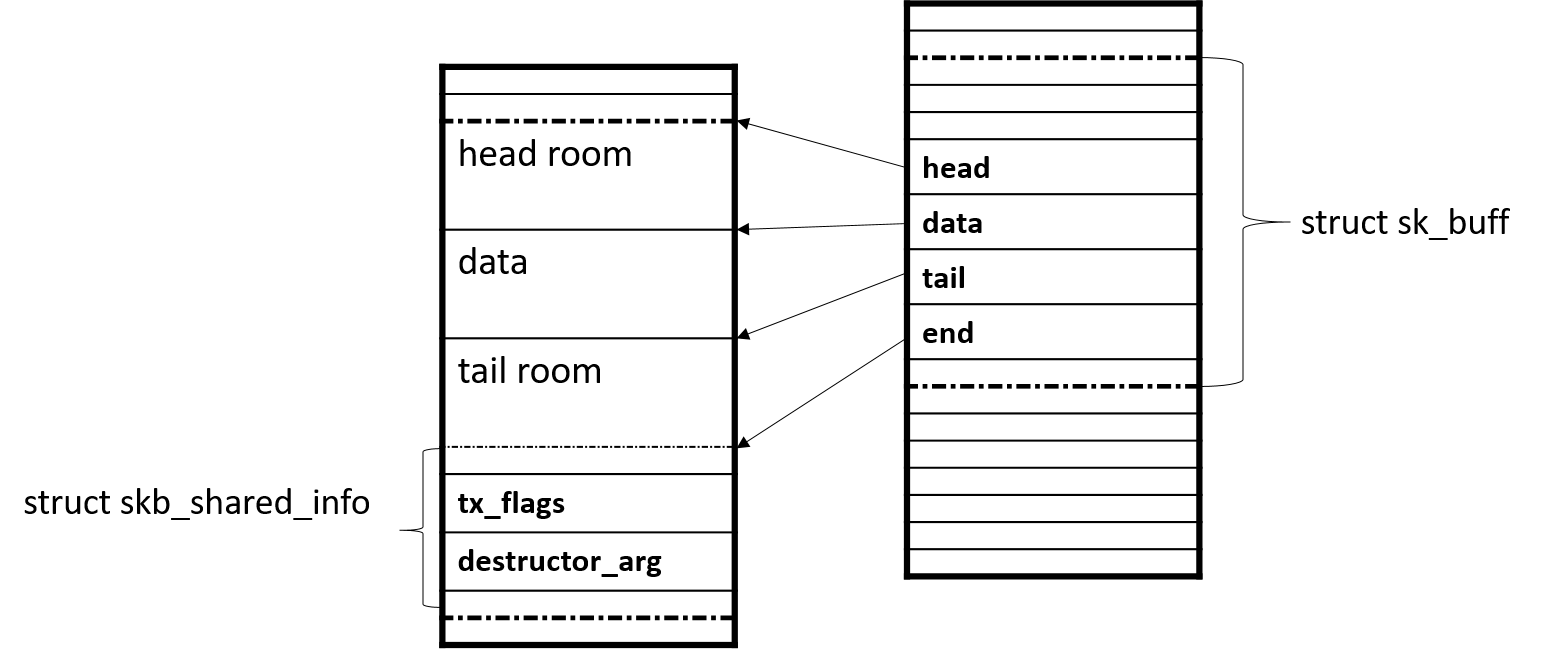
\includegraphics[width=1.2\linewidth]{figs/skb.png}
    \caption{\texttt{struct sk\_buff} and \shinfo}
    \label{fig:sh_info}
\end{figure}

\subsection{\shinfo co-location}
Additional challenge with attacking \shinfo is the fact the the fields are filled and rewritten by the device driver; after the packet is received. As it turns out this is not a problem as multiple device drivers \footnote{make sure to get list from Gil's Thesis} first create an skb and only then unmap, allowing the device ample opportunity to annul the changes made by the driver. But even when the order is correct; the default mode in Linux us deferred protection and although the page was unmapped the device can still access it via the IOTLB. Still, in the case when the strict protection is used; the device can rewrite \shinfo due to the way \shinfo is allocated. An RX skb is allocated via the \texttt{napi\_alloc\_skb} function\footnote{there are several other options as well, but the principle is the same} this function uses a page frag to allocate the \texttt{data} buffer that contains \shinfo. While, it is possible that the iova we were using has been invalidated, we can still access the physical page using the iova of the next RX descriptor.
\begin{figure*}[t]
                \begin{lstlisting}[
        %basicstyle = \scriptsize,
        columns = space-flexible,
        tabsize=8,
        %frame = l,
        language = C
        ]
#define __va(x) ((void *)((unsigned long) (x)))
#define __pa(x) ((unsigned long) (x))

#define virt_to_pfn(kaddr)      (__pa(kaddr) >> PAGE_SHIFT)
#define pfn_to_virt(pfn)        __va((pfn) << PAGE_SHIFT)

        /* memmap is virtually contiguous.  */
#define __pfn_to_page(pfn)      (vmemmap + (pfn))  
#define __page_to_pfn(page)     (unsigned long)((page) - vmemmap)
                \end{lstlisting}
        \caption{ The transition between KVA, PFN and \page is just a matter of shifting bits.
                }
        \label{fig:mem_model}
\end{figure*}
\subsection{Ring Flod}
To execute a successful DMA attack on an writable callback pointer; the attacking device needs a memory buffer filled with malicious code and the kernel address of that buffer.
Every RX packet is a possible buffer of malicious code, but the device is only given the buffer iova. The mapping between an iova and its kva is held in the device page table and the device driver meta-data; neither is accessible to the device. Additionally the \texttt{struct page} address is filled by the driver(not the KVA) on RX but while we have write access we don't have read access. The current memory model of x86-64 and ARM Linux servers is SPARSEMEM\_VMEMMAP \cite{mem_model}. Under this memory model the transition between KVA,PFN and \page is trivial once we have the vmem\_base value (Fig \ref{fig:mem_model}).\newline 
The boot process is deterministic; executing the same set of commands, initiating the same modules and allocating the same amount of memory each reboot. While the actual pages each module gets will vary in a multi-core machine due to timing issues, the drift is not expected to be to large. We evaluate this assumptions running 128 reboots on three Dell machines with different kernel versions. In the fig\footnote{Please generate figure of RingFlod Results} we show the memory used by each driver and how many of the pfns repeat in more than X\% percent. Thus an adversary that has some knowledge about the physical setup and the kernel being used can guess with a high probability a valid kva for one of the RX pages. Whats left is to fill all the pages with a valid uarg struct with a callback pointer set back to it self, see fig \footnote{Need to generate a fig of a valid \uarg}.

\subsection{Privilege escalation}
\shinfo of a TX packet is read only to the NIC.
But if the fragments hold malicious content; its all the malicious NIC needs for a successful attack. The readable \shinfo holds a \kva for a \page. This both allows the NIC to break KASLR and gives a \kva of a valid \mabaf. \textcolor{red}{Under the assumptions of a memory model its straightforward to calculate a \kva}.\footnote{complete the memory model info and calculation}. To implement the attack the NIC will generate an RX packet and will fill the \uarg address from the calculated \kva.
The NIC will hold off on the TX completion event in order to make sure that \kva is not freed in the completion handler; before the poisoned RX packet is processed. A TX completion event that fails to appear will trigger a TX T/O error that will flush all buffers; the T/O is set by the driver usually to 5 seconds, which is enough to implement an attack.\newline
In this scenario the attacker doesn't need any prior knowledge of the kernel or the hardware. The only assumption is that there is an accomplice that can open a socket in user-space or even in user-space of a guest machine; making any cloud VM a valid intrusion tool.

\subsection{Packet Forwarding}
Packet forwarding functionality is usualy disabled by default in Linux machines. But some Linux servers may function as a router or a load balancer; these machines will have packet forwarding enabled. In this scenario the NIC can independently generate an RX packets with a \mabaf. These packets can have valid 5 tuples to their network. The driver will complete the \page address of the buffer. \textcolor{red}{These packets will be forwarded and so become a TX packet that can be used as described in the previous attack.} \footnote{Need to check what happens to sh\_info, can we just forward a packet with frags (MTU, is usually a limiting factor)}

\subsubsection{When page frags are used indiscriminately}
\textcolor{magenta}{Unfortunately the following is not found in nature... - XDP Does :)}\newline
In case where both TX and RX sh\_info come from the same page frag. The NIC can read arbitrary kernel addresses by modifying the frag list of a TX skb thus making the driver map random addresses.
Being able to read the \shinfo, allows the NIC to generate an RX packet packet with \mabaf; the \kva of which will be written by driver and read by the NIC via TX iova. From this point and on we refer the reader to the steps in the previous sections.
\subsection{XDP}
\textcolor{red}{XDP (5.1.12)is not umpapping or using DMA\_MAP\_BIDIR \- please show its ill advised...} The linear skbs in mlx5 are mapping sh\_info as BI\_DIR, need to see when linear used vs non-linear and to check othe XDP drivers. When sh\_info is mapped BI\_DIR its all we need to attack. 